\documentclass[conference]{IEEEtran}
\IEEEoverridecommandlockouts

\usepackage{cite}
\usepackage{amsmath,amssymb,amsfonts}
\usepackage{algorithmic}
\usepackage{graphicx}
\usepackage{textcomp}
\usepackage{xcolor}
\usepackage{booktabs}
\usepackage{microtype}

\def\BibTeX{{\rm B\kern-.05em{\sc i\kern-.025em b}\kern-.08em
    T\kern-.1667em\lower.7ex\hbox{E}\kern-.125emX}}

\begin{document}

\title{EffiNIDS: A Computation-Aware Feature Selection Approach for High-Performance Network Intrusion Detection Systems}

\author{
\IEEEauthorblockN{Sayeed Ibne Saif}
\IEEEauthorblockA{\textit{Department of Computer Science and Engineering} \\
\textit{Premier University}\\
Chattogram-4000, Bangladesh \\
sayeedibnesaif123@gmail.com}
\and
\IEEEauthorblockN{Md. Azmayen}
\IEEEauthorblockA{\textit{Department of Computer Science and Engineering} \\
\textit{Premier University}\\
Chattogram-4000, Bangladesh \\
mdazmayen@outlook.com}
\and
\IEEEauthorblockN{Nusrath Saqi}
\IEEEauthorblockA{\textit{Department of Computer Science and Engineering} \\
\textit{Premier University}\\
Chattogram-4000, Bangladesh \\
nusrathsaqi@gmail.com}
}

\maketitle

\begin{abstract}
Machine learning-based Network Intrusion Detection Systems (NIDS) must process high-volume network traffic in near real time. However, raw traffic flows generate dozens of statistical and protocol features. High input dimensionality increases both training overhead and per-packet classification latency, creating bottlenecks for resource-constrained edge routers and security appliances. This paper presents EffiNIDS, an empirical evaluation framework investigating whether feature reduction can reduce computational costs while preserving attack detection accuracy. Using the UNSW-NB15 benchmark dataset (257,673 records), we evaluate two feature selection paradigms: Mutual Information (a filter method) and Random Forest impurity importance (an embedded method). Both methods reduce the 194 one-hot encoded features by 50\% down to 97 features. Experimental results show that a 50\% feature cut produces no loss in detection performance: test accuracy remains 87.19\% (compared to 87.09\% baseline), attack F1-score reaches 89.45\% (versus 89.38\% baseline), and inference latency drops by up to 15.1\%. In addition, a diagnostic pattern analysis reveals that 89.6\% of test records contain feature patterns never encountered during training, where the model maintains an 88.12\% attack F1-score. We also uncover 526 test records with conflicting labels for identical feature vectors, explaining a source of unavoidable test error within the UNSW-NB15 benchmark.
\end{abstract}

\begin{IEEEkeywords}
Network intrusion detection, feature selection, Random Forest, UNSW-NB15, computational efficiency, pattern consistency.
\end{IEEEkeywords}

\section{Introduction}
Modern computer networks face continuous, sophisticated cyber attacks, including distributed denial-of-service (DoS), remote exploits, fuzzing probes, and stealthy reconnaissance scans \cite{moustafa2015unsw}. Network Intrusion Detection Systems (NIDS) serve as a primary line of defense by inspecting network packets and connection flows to distinguish benign traffic from malicious activity \cite{ahmad2021network}. To keep pace with novel attack vectors, security teams increasingly rely on machine learning models capable of identifying behavioral traffic anomalies without manual signature authoring \cite{thakkar2022review}.

However, practical deployment introduces severe resource constraints. In high-speed campus networks, enterprise firewalls, and IoT gateways, traffic inspection must occur within strict timing budgets \cite{sarhan2022towards}. Raw network flow extractors capture dozens of attributes per connection, ranging from connection duration and byte counts to TCP window advertisements and inter-arrival jitter \cite{moustafa2016evaluation}. When categorical attributes such as protocols and connection states are one-hot encoded, the input feature space expands rapidly. Passing hundreds of features to an ensemble model increases memory consumption, slows down real-time packet classification, and wastes CPU cycles on uninformative or redundant inputs \cite{janarthanan2017feature}.

A common response in the literature is feature selection \cite{guyon2003introduction}. Yet, existing NIDS papers typically focus on classification accuracy while overlooking the end-to-end computational budget \cite{kasongo2020performance}. A feature selection method that saves 5\% in inference time is counterproductive if selecting those features requires hours of compute time. Conversely, an upfront selection step that requires modest training overhead can yield compound latency savings when deployed over billions of production packets.

This paper addresses that trade-off through \textbf{EffiNIDS}, an experimental framework that evaluates feature reduction, detection performance, and computational overhead under identical pipeline conditions. Using the official UNSW-NB15 training and test partitions, we compare a full-feature baseline against two selection strategies: Mutual Information (MI), a model-agnostic filter method, and Random Forest (RF) Mean Decrease in Impurity (MDI), an embedded method. Each approach discards exactly 50\% of the encoded features (retaining 97 out of 194).

Beyond standard metric comparisons, this study investigates model behavior under two practical conditions. First, we examine model robustness when confronted with traffic patterns never seen during training. Second, we audit the dataset for identical flow patterns that carry contradictory ground-truth labels.

The primary contributions of this work are:
\begin{enumerate}
    \item We compare filter-based (MI) and embedded (RF importance) feature selection on the UNSW-NB15 dataset under strict data leakage controls, where all preprocessing and selection steps fit exclusively on training data.
    \item We quantify the computational asymmetry between training overhead and inference speedup, showing that a 50\% feature cut reduces test inference latency by up to 15.1\% with negligible impact on model accuracy (87.19\% vs. 87.09\%).
    \item We evaluate generalization across 73,791 unseen flow patterns (89.6\% of test traffic), showing that the model maintains an 88.12\% attack F1-score on previously unencountered traffic signatures.
    \item We identify and quantify 526 conflicting records in UNSW-NB15 where identical flow features map to opposite labels, isolating an intrinsic data quality issue that caps achievable test accuracy.
\end{enumerate}

The remainder of this paper is structured as follows. Section II reviews related work. Section III presents the dataset, feature selection algorithms, and experimental pipeline. Section IV analyzes detection accuracy, computational costs, feature rankings, and pattern consistency. Section V discusses practical implications and limitations. Section VI concludes the paper.

\begin{figure*}[t]
\centerline{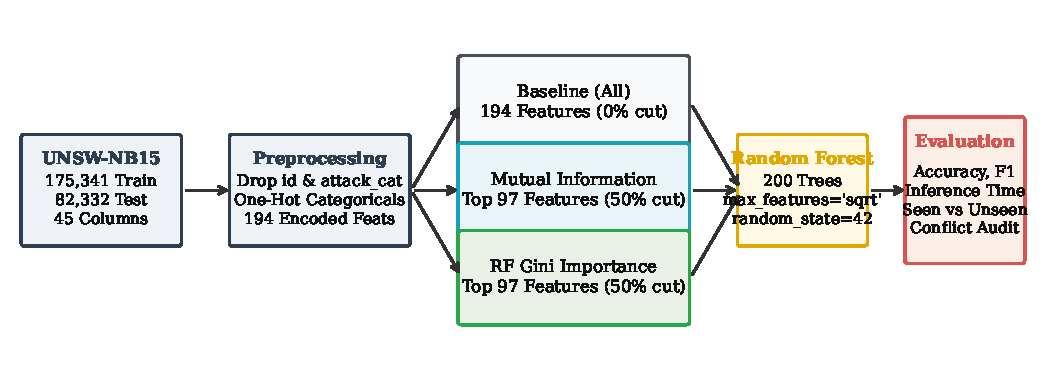
\includegraphics[width=0.92\textwidth]{figures/pipeline.pdf}}
\caption{The EffiNIDS experimental workflow. Preprocessing transformations and feature selectors are fitted exclusively on the 175,341 training records. The 82,332 test records are evaluated without modification.}
\label{fig:pipeline}
\end{figure*}

\section{Related Work}

\subsection{Machine Learning in Network Intrusion Detection}
Machine learning approaches for NIDS have progressed from legacy benchmarks such as KDD Cup 99 and NSL-KDD to modern datasets that reflect realistic protocol distributions and contemporary attack families \cite{sharafaldin2018toward}. Classifiers such as Naive Bayes, Support Vector Machines (SVM), Decision Trees, and Artificial Neural Networks (ANN) have been extensively benchmarked \cite{ahmad2021network}. 

Among classical algorithms, Random Forest \cite{breiman2001random} has emerged as an effective choice for tabular network flow data. Belouch et al. \cite{belouch2018performance} evaluated Random Forest against alternative classifiers on Apache Spark and observed superior F1-scores and robustness against overfitting. Similarly, Al-Zewairi et al. \cite{alzewairi2017experimental} evaluated multi-layer perceptrons on UNSW-NB15, finding that deep architectures require careful regularization to match tree-based ensembles on tabular network flows.

\subsection{Feature Selection in NIDS}
Feature selection techniques are categorized into filter, wrapper, and embedded methods \cite{guyon2003introduction}. Filter methods evaluate individual feature relevance using statistical properties independent of the downstream classifier. Ambusaidi et al. \cite{ambusaidi2016building} proposed a mutual information-based feature selection algorithm (FMIFS) that removed redundant attributes before training an LS-SVM classifier, achieving high accuracy with reduced input dimensions.

Wrapper methods rely on classifier feedback to iteratively select optimal feature subsets. While wrappers often find compact subsets with high accuracy, their iterative nature demands high computational cost, making them impractical for large-scale datasets \cite{kasongo2020performance}. Embedded methods, such as tree-based impurity rankings and L1 regularization, integrate feature selection directly into model training. Kasongo and Sun \cite{kasongo2020performance} applied XGBoost-based feature selection to UNSW-NB15, demonstrating that reducing features from 42 to 19 improved Decision Tree accuracy from 85.56\% to 88.13\%.

\subsection{Studies on the UNSW-NB15 Benchmark}
Introduced by Moustafa and Slay in 2015 \cite{moustafa2015unsw}, the UNSW-NB15 dataset was generated with the IXIA PerfectStorm tool to address shortcomings of older benchmarks. The authors evaluated standard classifiers, reporting baseline accuracies between 75\% and 85\% \cite{moustafa2016evaluation}. Janarthanan and Zargari \cite{janarthanan2017feature} applied Information Gain and Correlation-based Feature Selection (CFS) to UNSW-NB15, showing that subset selection reduced processing time while retaining predictive accuracy. Kumar et al. \cite{kumar2020integrated} developed an integrated rule-based framework combining feature clustering with ensemble classifiers.

Despite these studies, two gaps remain. First, most published evaluations do not measure the time required to perform feature selection alongside final training and test inference times. Second, standard evaluations report aggregate test metrics without examining whether the test partition contains flow patterns identical to the training set or flows with contradictory labels. EffiNIDS addresses both aspects directly.

\section{Methodology}

\subsection{Dataset and Preprocessing}
We use the official training and testing sets of the UNSW-NB15 dataset \cite{moustafa2015unsw}:
\begin{itemize}
    \item \textbf{Training set:} 175,341 records (56,000 normal, 119,341 attack).
    \item \textbf{Testing set:} 82,332 records (37,000 normal, 45,332 attack).
\end{itemize}
Each record contains 45 attributes. To ensure valid evaluation and avoid target leakage:
\begin{enumerate}
    \item The record identifier (`id`) was removed because it contains arbitrary row ordering without predictive value.
    \item The multiclass category attribute (`attack\_cat`) was removed from the predictor set. Retaining attack category descriptions during binary classification introduces target leakage.
\end{enumerate}
This leaves 42 input predictors: 39 continuous/discrete numerical features and 3 nominal categorical features (`proto`, `service`, and `state`).

The three categorical features were transformed using one-hot encoding via scikit-learn's `OneHotEncoder(handle_unknown="ignore")`. The transformation expanded the 3 categorical attributes into 155 binary indicator columns, while the 39 numerical features passed through unchanged. This yielded a total of \textbf{194 encoded input features}. All transformers were fitted exclusively on the training partition.

\subsection{Feature Selection Strategies}
We evaluate two selection techniques against the full 194-feature baseline:

\subsubsection{Mutual Information (MI) Selection}
Mutual Information quantifies the reduction in uncertainty about the binary class label $Y$ given knowledge of feature $X$:
\begin{equation}
I(X; Y) = \sum_{x \in \mathcal{X}} \sum_{y \in \mathcal{Y}} p(x, y) \log \frac{p(x, y)}{p(x)p(y)}
\label{eq:mi}
\end{equation}
For continuous numerical features, we estimate MI using non-parametric $k$-nearest neighbors entropy estimators based on the Kraskov-St\"ogbauer-Grassberger approach \cite{kraskov2004estimating}. Each of the 194 encoded features receives an individual MI score. The top 97 features (50\% cut) with the highest mutual information are retained. MI selection operates as a univariate filter: it requires no iterative tree fitting.

\subsubsection{Random Forest Impurity Importance Selection}
The embedded selection method uses Mean Decrease in Impurity (MDI). An initial Random Forest model with 200 trees is trained on all 194 features. For each feature $X_j$, its importance score $Imp(X_j)$ is computed as the total normalized reduction in Gini impurity brought by that feature across all split nodes in all trees:
\begin{equation}
Imp(X_j) = \frac{1}{N_T} \sum_{T} \sum_{t \in T: v(s_t) = X_j} p(t) \Delta i(s_t, t)
\label{eq:mdi}
\end{equation}
where $N_T$ is the number of trees, $p(t)$ is the proportion of samples reaching node $t$, and $\Delta i(s_t, t)$ is the impurity decrease produced by split $s_t$. All 194 features are ranked by MDI, and the top 97 features are selected. A second, final Random Forest is then trained exclusively on those selected 97 columns.

\subsection{Classifier Configuration}
All configurations employ the same core classifier: a Random Forest with 200 estimators, tree split criterion based on Gini impurity, maximum features per split set to $\sqrt{p}$ (where $p$ is the number of active features), and a fixed random seed (`random_state=42`). Computations ran in parallel using all available CPU threads (`n_jobs=-1`).

\subsection{Evaluation Metrics and Execution Environment}
Model quality was assessed using standard binary classification metrics:
\begin{align}
\text{Accuracy} &= \frac{TP + TN}{TP + TN + FP + FN} \\
\text{Attack Recall} &= \frac{TP}{TP + FN} \\
\text{Precision} &= \frac{TP}{TP + FP} \\
\text{Attack F1} &= \frac{2 \cdot \text{Precision} \cdot \text{Recall}}{\text{Precision} + \text{Recall}} \\
\text{False Positive Rate (FPR)} &= \frac{FP}{FP + TN}
\end{align}
where $TP$, $TN$, $FP$, and $FN$ represent true positives, true negatives, false positives, and false negatives, with Attack designated as the positive class ($1$).

Computational efficiency was evaluated across two dimensions:
\begin{itemize}
    \item \textbf{Training and Selection Time:} The total wall-clock seconds required to perform feature ranking, feature subset extraction, and final model fitting.
    \item \textbf{Inference Latency:} The median wall-clock time across three full test runs over all 82,332 records, normalized to milliseconds per connection record.
\end{itemize}
All experiments ran on a 64-bit Windows 11 host equipped with an AMD Ryzen 5 5600G processor (6 cores, 12 threads @ 3.90 GHz) and 16 GB of DDR4 RAM.

\section{Results and Analysis}

\subsection{Detection Performance Comparison}
Table~\ref{tab:performance} summarizes classification performance across the 82,332 test records. Figure~\ref{fig:comparison_bar} visualizes the metrics, and Fig.~\ref{fig:confusion_matrix} displays the corresponding confusion matrices.

\begin{table}[htbp]
\caption{Classification Performance on the UNSW-NB15 Test Set (82,332 Records)}
\begin{center}
\begin{tabular}{lcccccc}
\toprule
\textbf{Configuration} & \textbf{Feats} & \textbf{Acc (\%)} & \textbf{Rec (\%)} & \textbf{F1 (\%)} & \textbf{MF1 (\%)} & \textbf{FPR (\%)} \\
\midrule
Baseline RF & 194 & 87.09 & 98.63 & 89.38 & 86.46 & 27.05 \\
MI Selection & 97 & 87.15 & 98.55 & 89.41 & 86.53 & 26.82 \\
\textbf{RF Importance} & \textbf{97} & \textbf{87.19} & \textbf{98.56} & \textbf{89.45} & \textbf{86.58} & \textbf{26.73} \\
\bottomrule
\multicolumn{7}{l}{\footnotesize Feats = Features; Acc = Accuracy; Rec = Attack Recall; F1 = Attack F1;} \\
\multicolumn{7}{l}{\footnotesize MF1 = Macro-F1; FPR = False Positive Rate.}
\end{tabular}
\label{tab:performance}
\end{center}
\end{table}

\begin{figure}[htbp]
\centerline{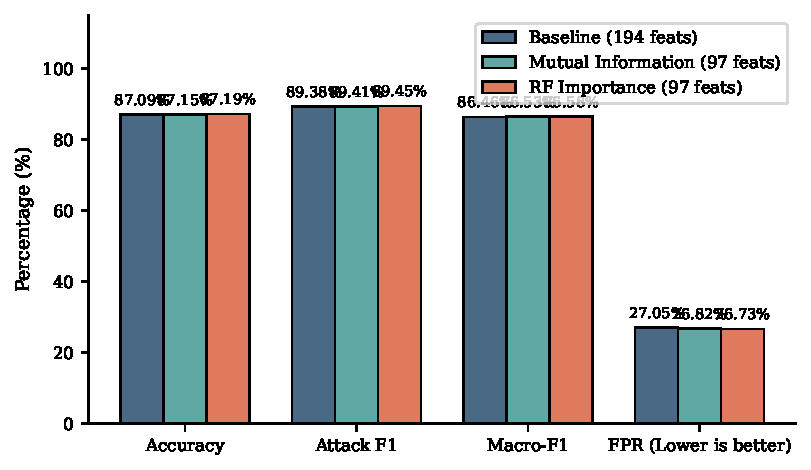
\includegraphics[width=0.98\columnwidth]{figures/comparison_bar.pdf}}
\caption{Detection performance comparison across the three configurations. Removing 50\% of input features slightly improves accuracy and lowers FPR.}
\label{fig:comparison_bar}
\end{figure}

\begin{figure*}[t]
\centerline{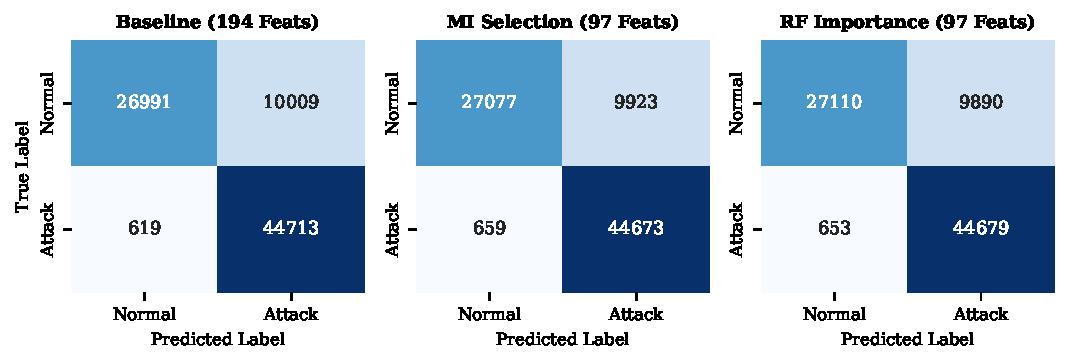
\includegraphics[width=0.95\textwidth]{figures/confusion_matrix.pdf}}
\caption{Confusion matrices for Baseline (194 features), Mutual Information (97 features), and RF Importance (97 features) on the test set.}
\label{fig:confusion_matrix}
\end{figure*}

The experimental results show that eliminating 50\% of the input features caused no degradation in detection accuracy. The baseline Random Forest using all 194 features attained 87.09\% accuracy and an attack F1-score of 89.38\%. Selecting 97 features via Mutual Information nudged accuracy to 87.15\% and F1 to 89.41\%. RF Importance selection achieved the highest overall metrics: 87.19\% accuracy, 89.45\% attack F1-score, and 86.58\% Macro-F1. 

In addition, false positive rates decreased from 27.05\% in the baseline model to 26.82\% under MI selection and 26.73\% under RF Importance. By discarding 97 redundant one-hot protocol indicators, the classifiers avoided spurious decision splits on rare categories, producing modest gains in generalization.

\subsection{Computational Cost and Trade-off Analysis}
Table~\ref{tab:timing} reports the computational cost profile. The data reveals an operational trade-off between upfront model creation time and subsequent classification speed.

\begin{table}[htbp]
\caption{Computational Cost Profile and Inference Latency}
\begin{center}
\begin{tabular}{lcccc}
\toprule
\textbf{Configuration} & \textbf{Train+Select (s)} & \textbf{Inference (s)} & \textbf{ms/Record} & \textbf{$\Delta$ Inf (\%)} \\
\midrule
Baseline RF & 61.28 & 0.516 & 0.00626 & --- \\
MI Selection & 75.26 & \textbf{0.438} & \textbf{0.00532} & \textbf{$-$15.11\%} \\
RF Importance & 124.76 & 0.474 & 0.00576 & $-$8.14\% \\
\bottomrule
\multicolumn{5}{l}{\footnotesize Train+Select = Total training plus selection time; ms/Record = Latency per record;} \\
\multicolumn{5}{l}{\footnotesize $\Delta$ Inf = Percentage change in test inference latency relative to baseline.}
\end{tabular}
\label{tab:timing}
\end{center}
\end{table}

\begin{itemize}
    \item \textbf{Training Phase:} Baseline training required 61.28 seconds. MI feature selection added a modest 22.8\% overhead, completing in 75.26 seconds because mutual information scores are computed directly between individual features and labels. In contrast, RF Importance required 124.76 seconds (+103.6\%) because an initial 200-tree model had to be fully trained first to extract impurity scores before training the final classifier.
    \item \textbf{Inference Phase:} Both feature-reduced models yielded faster test inference across the 82,332 records. The baseline required 0.516 seconds (0.00626 ms per record). RF Importance reduced this to 0.474 seconds (an 8.14\% speedup). MI selection achieved the lowest latency at 0.438 seconds (0.00532 ms per record), representing a \textbf{15.11\% reduction} in classification time.
\end{itemize}

In an operational deployment where models are trained periodically (e.g., daily) but inspect millions of continuous flows, the 14-second training overhead of MI selection is offset by continuous latency savings during inspection.

\begin{figure*}[t]
\centerline{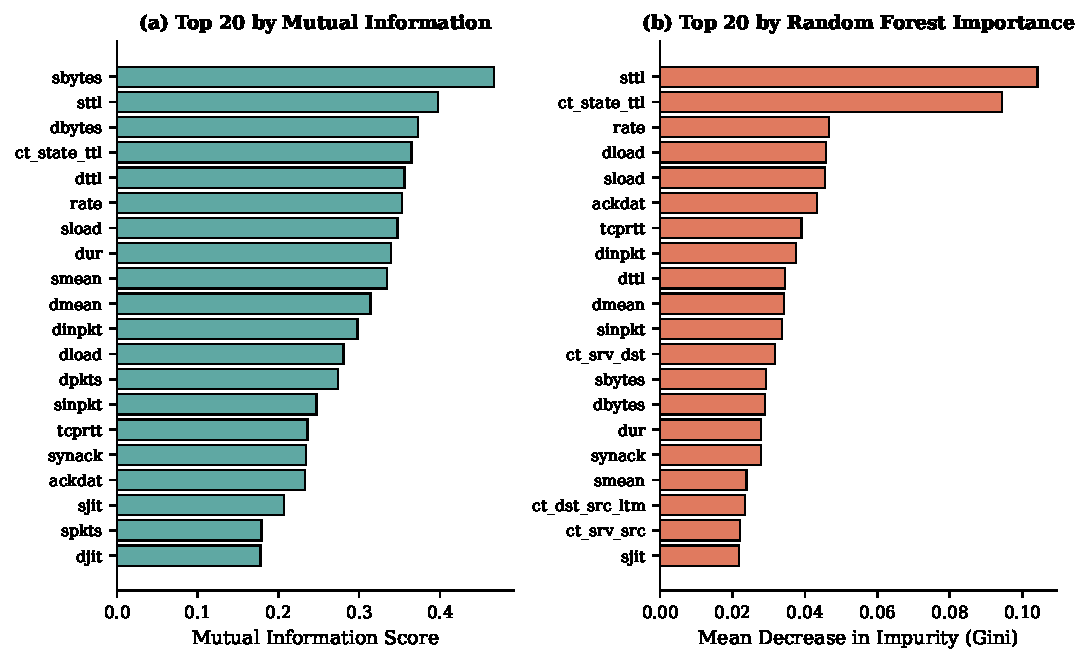
\includegraphics[width=0.95\textwidth]{figures/feature_importance.pdf}}
\caption{Side-by-side comparison of the top 20 features ranked by (a) Mutual Information score and (b) Random Forest Mean Decrease in Impurity.}
\label{fig:feature_importance}
\end{figure*}

\subsection{Feature Importance and Ranking Analysis}
Figure~\ref{fig:feature_importance} presents the top 20 features identified by each selection method. Both ranking strategies converge on specific traffic properties:
\begin{itemize}
    \item \textbf{Time-to-Live (TTL):} `sttl` (source TTL) and `dttl` (destination TTL) emerged as strong discriminators. `sttl` ranked second in MI (score 0.398) and first in RF Importance (weight 0.104). Attack tools and automated scanners often configure default or anomalous TTL header fields that diverge from legitimate host OS distributions.
    \item \textbf{Traffic Volume and Flow Rates:} `sbytes` (source byte volume, MI rank 1 with 0.467), `dbytes` (destination byte volume), `rate` (packet transmission rate), and `dload` (destination throughput) appear among the top positions in both rankings.
    \item \textbf{Connection State and Aggregation:} The composite attribute `ct\_state\_ttl` ranked fourth in MI (0.365) and second in RF Importance (0.094), confirming that combined connection state and TTL profiles capture multi-stage attack behavior.
\end{itemize}

Conversely, the bottom 97 features discarded by both methods consisted primarily of sparse one-hot encoded protocol columns (such as `proto_isis`, `proto_xns-idp`, `proto_iso-ip`, and `proto_hmp`), which had near-zero importance ($< 10^{-7}$). Removing these zero-information attributes simplified tree structures without losing predictive signal.

\subsection{Robustness Evaluation: Seen vs. Unseen Traffic}
A common criticism of benchmark evaluations is that high test scores may reflect memorization of repetitive flows rather than generalized pattern recognition. To examine this, we partitioned the 82,332 test records into two subsets based on whether the exact 42-predictor vector had appeared in the training partition:
\begin{itemize}
    \item \textbf{Seen Patterns:} 8,541 records (10.37\% of the test set).
    \item \textbf{Unseen Patterns:} 73,791 records (89.63\% of the test set).
\end{itemize}

Table~\ref{tab:robustness} summarizes model performance across these two partitions.

\begin{table}[htbp]
\caption{Model Generalization on Seen vs. Unseen Traffic Patterns}
\begin{center}
\begin{tabular}{llcccc}
\toprule
\textbf{Model} & \textbf{Subset} & \textbf{Records} & \textbf{Acc (\%)} & \textbf{F1 (\%)} & \textbf{FPR (\%)} \\
\midrule
Baseline & Seen & 8,541 & 94.43 & 96.73 & 31.11 \\
MI Selection & Seen & 8,541 & 94.43 & 96.73 & 31.11 \\
RF Importance & Seen & 8,541 & 94.40 & 96.72 & 31.25 \\
\midrule
Baseline & Unseen & 73,791 & 86.24 & 88.12 & 26.88 \\
MI Selection & Unseen & 73,791 & 86.30 & 88.16 & 26.64 \\
RF Importance & Unseen & 73,791 & \textbf{86.36} & \textbf{88.20} & \textbf{26.54} \\
\bottomrule
\end{tabular}
\label{tab:robustness}
\end{center}
\end{table}

On the 8,541 seen records, all models achieved $\sim$94.4\% accuracy and 96.7\% attack F1-score. Crucially, on the 73,791 records comprising completely novel feature combinations, the feature-reduced models maintained 86.36\% accuracy and an 88.20\% attack F1-score. This confirms that the Random Forest classifiers learned generalizable decision boundaries rather than memorized input instances.

\subsection{Diagnostic Analysis: Consistent vs. Conflicting Patterns}
Further auditing of the 8,541 seen records revealed a data quality characteristic in the benchmark. We partitioned the test traffic into three mutually exclusive categories:
\begin{enumerate}
    \item \textbf{Seen-Consistent (8,015 records, 9.73\%):} Records whose feature vector appeared in training with a consistent ground-truth label.
    \item \textbf{Seen-Conflicting (526 records, 0.64\%):} Records whose feature vector appeared in the dataset with contradictory ground-truth labels (tagged as Normal in some instances and Attack in others).
    \item \textbf{Unseen (73,791 records, 89.63\%):} Records whose feature combinations did not appear in training.
\end{enumerate}

Table~\ref{tab:consistency} reports the performance breakdown across these three subsets.

\begin{table}[htbp]
\caption{Classification Breakdown Across Consistent, Conflicting, and Unseen Subsets}
\begin{center}
\begin{tabular}{llcccc}
\toprule
\textbf{Model} & \textbf{Subset} & \textbf{Records} & \textbf{Acc (\%)} & \textbf{F1 (\%)} & \textbf{FPR (\%)} \\
\midrule
Baseline & Seen-Consistent & 8,015 & \textbf{100.0} & \textbf{100.0} & \textbf{0.00} \\
MI Selection & Seen-Consistent & 8,015 & \textbf{100.0} & \textbf{100.0} & \textbf{0.00} \\
RF Importance & Seen-Consistent & 8,015 & \textbf{100.0} & \textbf{100.0} & \textbf{0.00} \\
\midrule
Baseline & Seen-Conflicting & 526 & 9.51 & 2.86 & 91.42 \\
MI Selection & Seen-Conflicting & 526 & 9.51 & 2.86 & 91.42 \\
RF Importance & Seen-Conflicting & 526 & 9.13 & 2.85 & 91.82 \\
\midrule
Baseline & Unseen & 73,791 & 86.24 & 88.12 & 26.88 \\
MI Selection & Unseen & 73,791 & 86.30 & 88.16 & 26.64 \\
RF Importance & Unseen & 73,791 & 86.36 & 88.20 & 26.54 \\
\bottomrule
\end{tabular}
\label{tab:consistency}
\end{center}
\end{table}

On the 8,015 seen-consistent records, all three models achieved \textbf{100.0\% accuracy and 100.0\% F1-score with 0.0\% FPR}. The models recalled consistent training patterns without error.

However, on the 526 conflicting records, accuracy dropped to 9.1\%--9.5\%, with false positive rates exceeding 91\%. When two flows possess identical feature values across all 42 input dimensions but carry opposing ground-truth tags, no deterministic classifier can label both correctly. This diagnostic isolates an inherent labeling ambiguity within UNSW-NB15, demonstrating that a fraction of test set misclassifications stem from benchmark data noise rather than model failure.

\section{Discussion and Limitations}

\subsection{Operational Considerations}
The experimental results demonstrate that feature selection provides practical advantages for high-throughput NIDS:
\begin{itemize}
    \item \textbf{Inference Speedup:} A 15.1\% reduction in inference time translates to higher packet processing throughput on edge hardware, lowering CPU utilization during traffic bursts.
    \item \textbf{Filter vs. Embedded Trade-off:} While RF Importance yielded a marginal edge in accuracy (+0.04\%), Mutual Information achieved a larger inference speedup (15.1\% vs. 8.1\%) with less than half the training overhead (75 s vs. 125 s). For operational environments that retrain frequently, filter-based MI selection offers the superior cost-to-benefit profile.
\end{itemize}

\subsection{The False Positive Rate Challenge}
Across all models, the false positive rate remained around 26.7\%--27.0\%. In a Security Operations Center (SOC) processing millions of events daily, an FPR of 27\% generates substantial alert fatigue. This elevated FPR occurs because certain normal connection sequences share behavioral attributes (e.g., high packet rates, short durations) with scanning and probe attacks. Mitigating this issue requires threshold calibration (shifting classification probability thresholds above 0.5), cost-sensitive loss formulations, or secondary alert-triage stages.

\subsection{Threats to Validity and Limitations}
Several limitations should be noted:
\begin{itemize}
    \item \textbf{Classifier Diversity:} The current study focuses on Random Forest. While Random Forest is a standard baseline for tabular network data, evaluating gradient boosting (XGBoost, LightGBM, CatBoost) and neural architectures remains necessary to confirm broader algorithm generality.
    \item \textbf{Dataset Scope:} Experiments were conducted on UNSW-NB15. Testing across secondary benchmarks, such as CIC-IDS2017, will help evaluate cross-environment feature stability.
    \item \textbf{Reduction Granularity:} We evaluated a single 50\% reduction threshold. Sweeping reduction ratios from 10\% to 90\% would map the full Pareto frontier between dimensionality and detection accuracy.
    \item \textbf{Single-Seed Evaluation:} Training and inference runtimes were measured on a single workstation with fixed random initialization. Multi-seed evaluations with formal statistical significance tests (e.g., Wilcoxon signed-rank tests) will further strengthen runtime claims.
\end{itemize}

\section{Conclusion and Future Work}
This paper introduced EffiNIDS, an empirical evaluation framework assessing the trade-off between feature reduction, detection quality, and computational cost in network intrusion detection. Benchmarked on the UNSW-NB15 dataset, our results show that discarding 50\% of one-hot encoded features (from 194 to 97) via Mutual Information or Random Forest Gini importance preserves detection efficacy. Test accuracy reached 87.19\% with an attack F1-score of 89.45\%, while per-record inference latency decreased by up to 15.11\%.

Our post-hoc pattern analysis further demonstrated that the model generalizes robustly across 73,791 previously unencountered traffic signatures (88.20\% F1-score), while achieving 100\% accuracy on consistent recurring flows. Finally, identifying 526 records with contradictory labels clarifies a source of residual error inherent to the UNSW-NB15 benchmark.

Future work will expand this framework across multiple classifiers (XGBoost, LightGBM, and TabNet), incorporate cross-dataset validation on CIC-IDS2017, evaluate multi-class attack categorization, and explore probability threshold calibration to lower operational false positive rates.

\begin{thebibliography}{15}

\bibitem{moustafa2015unsw}
N.~Moustafa and J.~Slay, ``{UNSW-NB15}: a comprehensive data set for network intrusion detection systems ({UNSW-NB15} network data set),'' in \emph{Proc. 2015 Military Communications and Information Systems Conference (MilCIS)}, 2015, pp. 1--6.

\bibitem{moustafa2016evaluation}
N.~Moustafa and J.~Slay, ``The evaluation of Network Anomaly Detection Systems: Features of the {UNSW-NB15} data set,'' \emph{Information Security Journal: A Global Perspective}, vol.~25, no. 1--3, pp. 120--134, 2016.

\bibitem{janarthanan2017feature}
T.~Janarthanan and S.~Zargari, ``Feature selection in {UNSW-NB15} and {KDDCUP'99} datasets,'' in \emph{Proc. 2017 IEEE 26th International Symposium on Industrial Electronics (ISIE)}, 2017, pp. 1881--1886.

\bibitem{kasongo2020performance}
S.~M. Kasongo and Y.~Sun, ``Performance analysis of intrusion detection systems using a feature selection method on the {UNSW-NB15} dataset,'' \emph{Journal of Big Data}, vol.~7, no.~1, pp. 1--20, 2020.

\bibitem{kumar2020integrated}
V.~Kumar, D.~Sinha, A.~K. Das, S.~C. Pandey, and R.~T. Goswami, ``An integrated rule-based intrusion detection system: analysis on {UNSW-NB15} data set and the real time online dataset,'' \emph{Cluster Computing}, vol.~23, pp. 1397--1418, 2020.

\bibitem{sarhan2022towards}
M.~Sarhan, S.~Layeghy, and M.~Portmann, ``Towards a standard feature set for network intrusion detection system datasets,'' \emph{Mobile Networks and Applications}, vol.~27, pp. 357--370, 2022.

\bibitem{sharafaldin2018toward}
I.~Sharafaldin, A.~H. Lashkari, and A.~A. Ghorbani, ``Toward generating a new intrusion detection dataset and intrusion traffic characterization,'' in \emph{Proc. 4th International Conference on Information Systems Security and Privacy (ICISSP)}, 2018, pp. 108--116.

\bibitem{guyon2003introduction}
I.~Guyon and A.~Elisseeff, ``An introduction to variable and feature selection,'' \emph{Journal of Machine Learning Research}, vol.~3, pp. 1157--1182, 2003.

\bibitem{breiman2001random}
L.~Breiman, ``Random forests,'' \emph{Machine Learning}, vol.~45, no.~1, pp. 5--32, 2001.

\bibitem{ambusaidi2016building}
M.~A. Ambusaidi, X.~He, P.~Nanda, and Z.~Tan, ``Building an intrusion detection system using a filter-based feature selection algorithm,'' \emph{IEEE Transactions on Computers}, vol.~65, no.~10, pp. 2986--2998, 2016.

\bibitem{ahmad2021network}
Z.~Ahmad, A.~S. Khan, C.~W. Shiang, J.~Abdullah, and F.~Ahmad, ``Network intrusion detection system: A systematic study of machine learning and deep learning approaches,'' \emph{Transactions on Emerging Telecommunications Technologies}, vol.~32, no.~1, p. e4150, 2021.

\bibitem{belouch2018performance}
M.~Belouch, S.~E. Hadaj, and M.~Idhammad, ``Performance evaluation of intrusion detection system using random forest on {Apache Spark},'' \emph{Procedia Computer Science}, vol. 127, pp. 1--6, 2018.

\bibitem{thakkar2022review}
A.~Thakkar and R.~Lohiya, ``A review on machine learning and deep learning perspectives of network intrusion detection systems,'' \emph{Archives of Computational Methods in Engineering}, vol.~29, no.~5, pp. 3219--3263, 2022.

\bibitem{alzewairi2017experimental}
M.~Al-Zewairi, S.~Almajali, and A.~Awajan, ``Experimental evaluation of a multi-layer perceptron for network intrusion detection on {UNSW-NB15},'' in \emph{Proc. 2017 8th International Conference on Information and Communication Systems (ICICS)}, 2017, pp. 165--170.

\bibitem{kraskov2004estimating}
A.~Kraskov, H.~St{\"o}gbauer, and P.~Grassberger, ``Estimating mutual information,'' \emph{Physical Review E}, vol.~69, no.~6, p. 066138, 2004.

\end{thebibliography}

\end{document}
